\documentclass{standalone}
\usepackage{tikz}
\usetikzlibrary{patterns, positioning}

\begin{document}
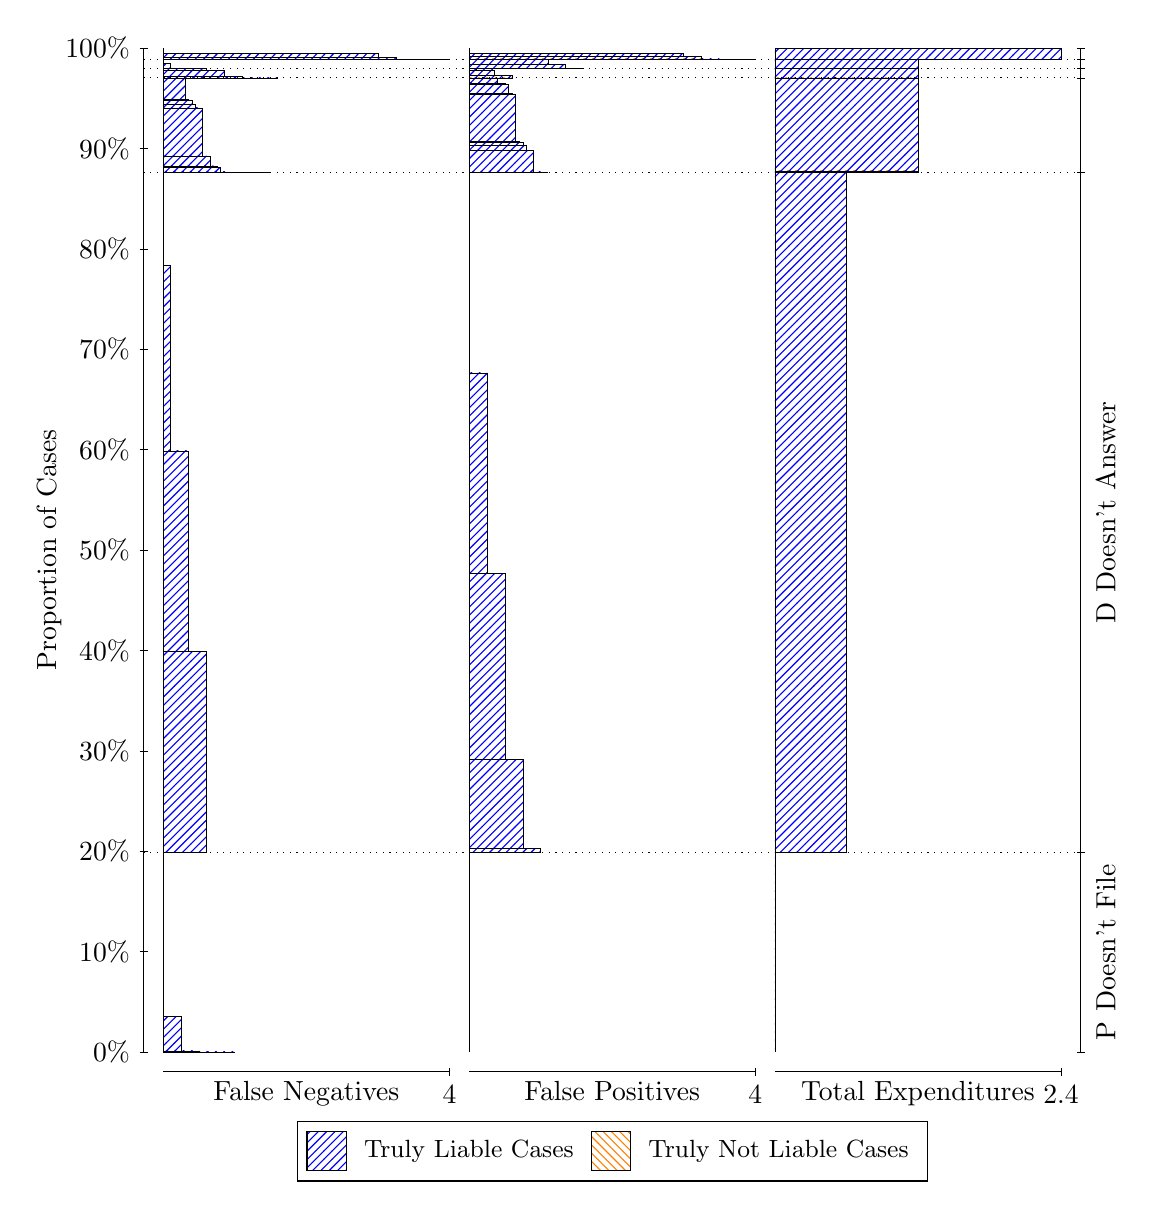
\begin{tikzpicture}
\draw[black, very thin] (1.5,1.75) -- (1.5,14.5);
\node[rotate=90, anchor=center] at (0.3, 8.125) {Proportion of Cases};
\draw[black, very thin] (1.45,1.75) -- (1.55,1.75);
\node[anchor=east] at (1.45, 1.75) {0\%};
\draw[black, very thin] (1.45,3.025) -- (1.55,3.025);
\node[anchor=east] at (1.45, 3.025) {10\%};
\draw[black, very thin] (1.45,4.3) -- (1.55,4.3);
\node[anchor=east] at (1.45, 4.3) {20\%};
\draw[black, very thin] (1.45,5.575) -- (1.55,5.575);
\node[anchor=east] at (1.45, 5.575) {30\%};
\draw[black, very thin] (1.45,6.85) -- (1.55,6.85);
\node[anchor=east] at (1.45, 6.85) {40\%};
\draw[black, very thin] (1.45,8.125) -- (1.55,8.125);
\node[anchor=east] at (1.45, 8.125) {50\%};
\draw[black, very thin] (1.45,9.4) -- (1.55,9.4);
\node[anchor=east] at (1.45, 9.4) {60\%};
\draw[black, very thin] (1.45,10.675) -- (1.55,10.675);
\node[anchor=east] at (1.45, 10.675) {70\%};
\draw[black, very thin] (1.45,11.95) -- (1.55,11.95);
\node[anchor=east] at (1.45, 11.95) {80\%};
\draw[black, very thin] (1.45,13.225) -- (1.55,13.225);
\node[anchor=east] at (1.45, 13.225) {90\%};
\draw[black, very thin] (1.45,14.5) -- (1.55,14.5);
\node[anchor=east] at (1.45, 14.5) {100\%};

\draw[black, very thin] (13.4,1.75) -- (13.4,14.5);
\draw[black, very thin] (13.35,1.75) -- (13.45,1.75);
\node[anchor=west] at (13.35, 1.75) {};
\draw[black, very thin] (13.35,4.2865) -- (13.45,4.2865);
\node[anchor=west] at (13.35, 4.2865) {};
\draw[black, very thin] (13.35,12.923) -- (13.45,12.923);
\node[anchor=west] at (13.35, 12.923) {};
\draw[black, very thin] (13.35,14.121) -- (13.45,14.121);
\node[anchor=west] at (13.35, 14.121) {};
\draw[black, very thin] (13.35,14.243) -- (13.45,14.243);
\node[anchor=west] at (13.35, 14.243) {};
\draw[black, very thin] (13.35,14.358) -- (13.45,14.358);
\node[anchor=west] at (13.35, 14.358) {};
\draw[black, very thin] (13.35,14.5) -- (13.45,14.5);
\node[anchor=west] at (13.35, 14.5) {};

\draw[black, very thin, pattern color=blue, pattern=north east lines] (1.75,1.75) rectangle (2.6583,1.75);
\draw[black, very thin, pattern color=blue, pattern=north east lines] (1.75,1.75) rectangle (2.4312,1.7501);
\draw[black, very thin, pattern color=blue, pattern=north east lines] (1.75,1.7501) rectangle (2.2042,1.7631);
\draw[black, very thin, pattern color=blue, pattern=north east lines] (1.75,1.7631) rectangle (1.9771,2.2061);
\draw[black, very thin, pattern color=orange, pattern=north west lines] (1.75,2.2061) rectangle (1.75,2.2061);
\draw[black, very thin, pattern color=blue, pattern=north east lines] (1.75,2.2061) rectangle (1.75,4.2865);
\draw[black, very thin, pattern color=blue, pattern=north east lines] (1.75,4.2865) rectangle (2.295,6.8364);
\draw[black, very thin, pattern color=blue, pattern=north east lines] (1.75,6.8364) rectangle (2.0679,9.3848);
\draw[black, very thin, pattern color=blue, pattern=north east lines] (1.75,9.3848) rectangle (1.8408,11.741);
\draw[black, very thin, pattern color=orange, pattern=north west lines] (1.75,11.741) rectangle (1.75,11.741);
\draw[black, very thin, pattern color=blue, pattern=north east lines] (1.75,11.741) rectangle (1.75,12.923);
\draw[black, very thin, pattern color=blue, pattern=north east lines] (1.75,12.923) rectangle (3.1125,12.923);
\draw[black, very thin, pattern color=blue, pattern=north east lines] (1.75,12.923) rectangle (3.0217,12.923);
\draw[black, very thin, pattern color=blue, pattern=north east lines] (1.75,12.923) rectangle (2.9308,12.923);
\draw[black, very thin, pattern color=blue, pattern=north east lines] (1.75,12.923) rectangle (2.8854,12.923);
\draw[black, very thin, pattern color=blue, pattern=north east lines] (1.75,12.923) rectangle (2.84,12.923);
\draw[black, very thin, pattern color=blue, pattern=north east lines] (1.75,12.923) rectangle (2.7946,12.923);
\draw[black, very thin, pattern color=blue, pattern=north east lines] (1.75,12.923) rectangle (2.7492,12.923);
\draw[black, very thin, pattern color=blue, pattern=north east lines] (1.75,12.923) rectangle (2.7037,12.923);
\draw[black, very thin, pattern color=blue, pattern=north east lines] (1.75,12.923) rectangle (2.6583,12.923);
\draw[black, very thin, pattern color=blue, pattern=north east lines] (1.75,12.923) rectangle (2.6129,12.923);
\draw[black, very thin, pattern color=blue, pattern=north east lines] (1.75,12.923) rectangle (2.5675,12.928);
\draw[black, very thin, pattern color=blue, pattern=north east lines] (1.75,12.928) rectangle (2.5221,12.928);
\draw[black, very thin, pattern color=blue, pattern=north east lines] (1.75,12.928) rectangle (2.4767,12.989);
\draw[black, very thin, pattern color=blue, pattern=north east lines] (1.75,12.989) rectangle (2.4312,12.997);
\draw[black, very thin, pattern color=blue, pattern=north east lines] (1.75,12.997) rectangle (2.3858,13.002);
\draw[black, very thin, pattern color=blue, pattern=north east lines] (1.75,13.002) rectangle (2.3404,13.123);
\draw[black, very thin, pattern color=blue, pattern=north east lines] (1.75,13.123) rectangle (2.295,13.131);
\draw[black, very thin, pattern color=blue, pattern=north east lines] (1.75,13.131) rectangle (2.2496,13.73);
\draw[black, very thin, pattern color=blue, pattern=north east lines] (1.75,13.73) rectangle (2.2042,13.741);
\draw[black, very thin, pattern color=blue, pattern=north east lines] (1.75,13.741) rectangle (2.1588,13.781);
\draw[black, very thin, pattern color=blue, pattern=north east lines] (1.75,13.781) rectangle (2.1133,13.841);
\draw[black, very thin, pattern color=blue, pattern=north east lines] (1.75,13.841) rectangle (2.0679,13.849);
\draw[black, very thin, pattern color=blue, pattern=north east lines] (1.75,13.849) rectangle (2.0225,14.119);
\draw[black, very thin, pattern color=blue, pattern=north east lines] (1.75,14.119) rectangle (1.9317,14.121);
\draw[black, very thin, pattern color=blue, pattern=north east lines] (1.75,14.121) rectangle (1.8408,14.121);
\draw[black, very thin, pattern color=orange, pattern=north west lines] (1.75,14.121) rectangle (1.75,14.121);
\draw[black, very thin, pattern color=blue, pattern=north east lines] (1.75,14.121) rectangle (3.2033,14.121);
\draw[black, very thin, pattern color=blue, pattern=north east lines] (1.75,14.121) rectangle (2.9762,14.121);
\draw[black, very thin, pattern color=blue, pattern=north east lines] (1.75,14.121) rectangle (2.7492,14.141);
\draw[black, very thin, pattern color=blue, pattern=north east lines] (1.75,14.141) rectangle (2.5221,14.214);
\draw[black, very thin, pattern color=blue, pattern=north east lines] (1.75,14.214) rectangle (2.295,14.243);
\draw[black, very thin, pattern color=orange, pattern=north west lines] (1.75,14.243) rectangle (1.75,14.243);
\draw[black, very thin, pattern color=blue, pattern=north east lines] (1.75,14.243) rectangle (2.295,14.243);
\draw[black, very thin, pattern color=blue, pattern=north east lines] (1.75,14.243) rectangle (2.0679,14.244);
\draw[black, very thin, pattern color=blue, pattern=north east lines] (1.75,14.244) rectangle (1.8408,14.304);
\draw[black, very thin, pattern color=orange, pattern=north west lines] (1.75,14.304) rectangle (1.75,14.304);
\draw[black, very thin, pattern color=blue, pattern=north east lines] (1.75,14.304) rectangle (1.75,14.358);
\draw[black, very thin, pattern color=blue, pattern=north east lines] (1.75,14.358) rectangle (5.3833,14.358);
\draw[black, very thin, pattern color=blue, pattern=north east lines] (1.75,14.358) rectangle (5.1563,14.358);
\draw[black, very thin, pattern color=blue, pattern=north east lines] (1.75,14.358) rectangle (4.9292,14.359);
\draw[black, very thin, pattern color=blue, pattern=north east lines] (1.75,14.359) rectangle (4.7021,14.381);
\draw[black, very thin, pattern color=blue, pattern=north east lines] (1.75,14.381) rectangle (4.475,14.429);
\draw[black, very thin, pattern color=blue, pattern=north east lines] (1.75,14.429) rectangle (4.2479,14.429);
\draw[black, very thin, pattern color=blue, pattern=north east lines] (1.75,14.429) rectangle (4.0208,14.429);
\draw[black, very thin, pattern color=blue, pattern=north east lines] (1.75,14.429) rectangle (1.8863,14.429);
\draw[black, very thin, pattern color=orange, pattern=north west lines] (1.75,14.429) rectangle (1.75,14.429);
\draw[black, very thin, pattern color=blue, pattern=north east lines] (1.75,14.429) rectangle (1.75,14.5);
\draw[black, very thin, pattern color=orange, pattern=north west lines] (5.6333,1.75) rectangle (5.6333,1.75);
\draw[black, very thin, pattern color=blue, pattern=north east lines] (5.6333,1.75) rectangle (5.6333,4.2865);
\draw[black, very thin, pattern color=orange, pattern=north west lines] (5.6333,4.2865) rectangle (6.5417,4.2865);
\draw[black, very thin, pattern color=blue, pattern=north east lines] (5.6333,4.2865) rectangle (6.5417,4.3359);
\draw[black, very thin, pattern color=blue, pattern=north east lines] (5.6333,4.3359) rectangle (6.3146,5.4691);
\draw[black, very thin, pattern color=blue, pattern=north east lines] (5.6333,5.4691) rectangle (6.0875,7.8249);
\draw[black, very thin, pattern color=blue, pattern=north east lines] (5.6333,7.8249) rectangle (5.8604,10.373);
\draw[black, very thin, pattern color=blue, pattern=north east lines] (5.6333,10.373) rectangle (5.6333,12.923);
\draw[black, very thin, pattern color=orange, pattern=north west lines] (5.6333,12.923) rectangle (6.6325,12.923);
\draw[black, very thin, pattern color=blue, pattern=north east lines] (5.6333,12.923) rectangle (6.6325,12.923);
\draw[black, very thin, pattern color=orange, pattern=north west lines] (5.6333,12.923) rectangle (6.5417,12.923);
\draw[black, very thin, pattern color=blue, pattern=north east lines] (5.6333,12.923) rectangle (6.5417,12.926);
\draw[black, very thin, pattern color=orange, pattern=north west lines] (5.6333,12.926) rectangle (6.4508,12.926);
\draw[black, very thin, pattern color=blue, pattern=north east lines] (5.6333,12.926) rectangle (6.4508,13.196);
\draw[black, very thin, pattern color=blue, pattern=north east lines] (5.6333,13.196) rectangle (6.4054,13.203);
\draw[black, very thin, pattern color=orange, pattern=north west lines] (5.6333,13.203) rectangle (6.36,13.203);
\draw[black, very thin, pattern color=blue, pattern=north east lines] (5.6333,13.203) rectangle (6.36,13.264);
\draw[black, very thin, pattern color=blue, pattern=north east lines] (5.6333,13.264) rectangle (6.3146,13.304);
\draw[black, very thin, pattern color=orange, pattern=north west lines] (5.6333,13.304) rectangle (6.2692,13.304);
\draw[black, very thin, pattern color=blue, pattern=north east lines] (5.6333,13.304) rectangle (6.2692,13.315);
\draw[black, very thin, pattern color=blue, pattern=north east lines] (5.6333,13.315) rectangle (6.2237,13.914);
\draw[black, very thin, pattern color=blue, pattern=north east lines] (5.6333,13.914) rectangle (6.1783,13.922);
\draw[black, very thin, pattern color=blue, pattern=north east lines] (5.6333,13.922) rectangle (6.1329,14.042);
\draw[black, very thin, pattern color=blue, pattern=north east lines] (5.6333,14.042) rectangle (6.0875,14.048);
\draw[black, very thin, pattern color=blue, pattern=north east lines] (5.6333,14.048) rectangle (6.0421,14.056);
\draw[black, very thin, pattern color=blue, pattern=north east lines] (5.6333,14.056) rectangle (5.9967,14.116);
\draw[black, very thin, pattern color=blue, pattern=north east lines] (5.6333,14.116) rectangle (5.9513,14.116);
\draw[black, very thin, pattern color=blue, pattern=north east lines] (5.6333,14.116) rectangle (5.9058,14.121);
\draw[black, very thin, pattern color=blue, pattern=north east lines] (5.6333,14.121) rectangle (5.8604,14.121);
\draw[black, very thin, pattern color=blue, pattern=north east lines] (5.6333,14.121) rectangle (5.815,14.121);
\draw[black, very thin, pattern color=blue, pattern=north east lines] (5.6333,14.121) rectangle (5.7696,14.121);
\draw[black, very thin, pattern color=blue, pattern=north east lines] (5.6333,14.121) rectangle (5.7242,14.121);
\draw[black, very thin, pattern color=blue, pattern=north east lines] (5.6333,14.121) rectangle (5.6787,14.121);
\draw[black, very thin, pattern color=blue, pattern=north east lines] (5.6333,14.121) rectangle (5.6333,14.121);
\draw[black, very thin, pattern color=orange, pattern=north west lines] (5.6333,14.121) rectangle (6.1783,14.121);
\draw[black, very thin, pattern color=blue, pattern=north east lines] (5.6333,14.121) rectangle (6.1783,14.15);
\draw[black, very thin, pattern color=blue, pattern=north east lines] (5.6333,14.15) rectangle (5.9513,14.223);
\draw[black, very thin, pattern color=blue, pattern=north east lines] (5.6333,14.223) rectangle (5.7242,14.243);
\draw[black, very thin, pattern color=blue, pattern=north east lines] (5.6333,14.243) rectangle (5.6333,14.243);
\draw[black, very thin, pattern color=orange, pattern=north west lines] (5.6333,14.243) rectangle (7.0867,14.243);
\draw[black, very thin, pattern color=blue, pattern=north east lines] (5.6333,14.243) rectangle (7.0867,14.244);
\draw[black, very thin, pattern color=blue, pattern=north east lines] (5.6333,14.244) rectangle (6.8596,14.297);
\draw[black, very thin, pattern color=blue, pattern=north east lines] (5.6333,14.297) rectangle (6.6325,14.357);
\draw[black, very thin, pattern color=blue, pattern=north east lines] (5.6333,14.357) rectangle (6.4054,14.358);
\draw[black, very thin, pattern color=blue, pattern=north east lines] (5.6333,14.358) rectangle (6.1783,14.358);
\draw[black, very thin, pattern color=orange, pattern=north west lines] (5.6333,14.358) rectangle (9.2667,14.358);
\draw[black, very thin, pattern color=blue, pattern=north east lines] (5.6333,14.358) rectangle (9.2667,14.358);
\draw[black, very thin, pattern color=orange, pattern=north west lines] (5.6333,14.358) rectangle (9.0396,14.358);
\draw[black, very thin, pattern color=blue, pattern=north east lines] (5.6333,14.358) rectangle (9.0396,14.358);
\draw[black, very thin, pattern color=orange, pattern=north west lines] (5.6333,14.358) rectangle (8.8125,14.358);
\draw[black, very thin, pattern color=blue, pattern=north east lines] (5.6333,14.358) rectangle (8.8125,14.362);
\draw[black, very thin, pattern color=orange, pattern=north west lines] (5.6333,14.362) rectangle (8.5854,14.362);
\draw[black, very thin, pattern color=blue, pattern=north east lines] (5.6333,14.362) rectangle (8.5854,14.398);
\draw[black, very thin, pattern color=blue, pattern=north east lines] (5.6333,14.398) rectangle (8.3583,14.429);
\draw[black, very thin, pattern color=blue, pattern=north east lines] (5.6333,14.429) rectangle (8.1313,14.429);
\draw[black, very thin, pattern color=blue, pattern=north east lines] (5.6333,14.429) rectangle (7.9042,14.429);
\draw[black, very thin, pattern color=blue, pattern=north east lines] (5.6333,14.429) rectangle (7.6771,14.429);
\draw[black, very thin, pattern color=orange, pattern=north west lines] (5.6333,14.429) rectangle (5.6333,14.429);
\draw[black, very thin, pattern color=blue, pattern=north east lines] (5.6333,14.429) rectangle (5.6333,14.5);
\draw[black, very thin, pattern color=orange, pattern=north west lines] (9.5167,1.75) rectangle (9.5167,1.75);
\draw[black, very thin, pattern color=blue, pattern=north east lines] (9.5167,1.75) rectangle (9.5167,4.2865);
\draw[black, very thin, pattern color=orange, pattern=north west lines] (9.5167,4.2865) rectangle (10.425,4.2865);
\draw[black, very thin, pattern color=blue, pattern=north east lines] (9.5167,4.2865) rectangle (10.425,12.923);
\draw[black, very thin, pattern color=orange, pattern=north west lines] (9.5167,12.923) rectangle (11.333,12.923);
\draw[black, very thin, pattern color=blue, pattern=north east lines] (9.5167,12.923) rectangle (11.333,12.939);
\draw[black, very thin, pattern color=orange, pattern=north west lines] (9.5167,12.939) rectangle (11.333,12.939);
\draw[black, very thin, pattern color=blue, pattern=north east lines] (9.5167,12.939) rectangle (11.333,14.121);
\draw[black, very thin, pattern color=orange, pattern=north west lines] (9.5167,14.121) rectangle (11.333,14.121);
\draw[black, very thin, pattern color=blue, pattern=north east lines] (9.5167,14.121) rectangle (11.333,14.243);
\draw[black, very thin, pattern color=orange, pattern=north west lines] (9.5167,14.243) rectangle (11.333,14.243);
\draw[black, very thin, pattern color=blue, pattern=north east lines] (9.5167,14.243) rectangle (11.333,14.358);
\draw[black, very thin, pattern color=orange, pattern=north west lines] (9.5167,14.358) rectangle (13.15,14.358);
\draw[black, very thin, pattern color=blue, pattern=north east lines] (9.5167,14.358) rectangle (13.15,14.5);
\draw[black, dotted] (1.5,4.2865) -- (13.4,4.2865);
\draw[black, dotted] (1.5,12.923) -- (13.4,12.923);
\draw[black, dotted] (1.5,14.121) -- (13.4,14.121);
\draw[black, dotted] (1.5,14.243) -- (13.4,14.243);
\draw[black, dotted] (1.5,14.358) -- (13.4,14.358);
\draw[black, very thin] (1.75,1.5) -- (5.3833,1.5);
\node[anchor=north] at (3.5667, 1.5) {False Negatives};
\draw[black, very thin] (5.3833,1.45) -- (5.3833,1.55);
\node[anchor=north] at (5.3833, 1.45) {4};

\draw[black, very thin] (5.6333,1.5) -- (9.2667,1.5);
\node[anchor=north] at (7.45, 1.5) {False Positives};
\draw[black, very thin] (9.2667,1.45) -- (9.2667,1.55);
\node[anchor=north] at (9.2667, 1.45) {4};

\draw[black, very thin] (9.5167,1.5) -- (13.15,1.5);
\node[anchor=north] at (11.333, 1.5) {Total Expenditures};
\draw[black, very thin] (13.15,1.45) -- (13.15,1.55);
\node[anchor=north] at (13.15, 1.45) {2.4};

\node[black, centered, rotate=90] at (13.72, 3.0183) {P Doesn't File};
\node[black, centered, rotate=90] at (13.72, 8.6049) {D Doesn't Answer};





\draw (7.449999999999999,1.5) node[draw=none] (baseCoordinate) {};
\begin{scope}[align=center]
        \matrix[scale=0.5, draw=black, below=0.5cm of baseCoordinate, nodes={draw}, column sep=0.1cm]{
            \node[rectangle, draw, minimum width=0.5cm, minimum height=0.5cm, pattern=north east lines, pattern color=blue] {}; &
            \node[draw=none, font=\small] (B) {Truly Liable Cases}; &
            \node[rectangle, draw, minimum width=0.5cm, minimum height=0.5cm, pattern=north west lines, pattern color=orange] {}; &
            \node[draw=none, font=\small] (B) {Truly Not Liable Cases}; \\
            };
\end{scope}

\end{tikzpicture}
\end{document}